% Felipe Bandeira da Silva
% 01/12/2013

\documentclass[paper=a4, fontsize=11pt]{article}

\usepackage[brazil]{babel}
\usepackage[utf8]{inputenc}
\usepackage{listings}
\usepackage{color}
\usepackage{amsthm}
\usepackage{graphicx}

\usepackage{schemabloc}
\usetikzlibrary{circuits}

\usepackage{tabularx,ragged2e,booktabs,caption}

\setlength{\parindent}{0pt}
\setlength{\parskip}{18pt}

\title{\textsc{Laboratório Transformadores\\O transformador trifásico de núcleo plano}}
\author{Felipe Bandeira da Silva\\1020942-X}
%\date{}

\begin{document}

\maketitle

%\newpage

%\begin{abstract}
\textit{Este laboratório tem como objetivo: Estudar a formação do transformador trifásico de núcleo plano. Aprender como se liga um transformador Triângulo-Triângulo, Triângulo-Estrela, Estrela-Estrela, Triângulo-Z.}
%\end{abstract}

\newpage

\tableofcontents

\newpage

\listoffigures

\newpage

\listoftables

%%%%%%%%%%%%%%%%%%%%%%%%%%%%%%%%%%%%%%%%%%%%%%%%%%%%%%%%%%%%%%%%%%%%%%%%%%%%%%%%
% fundamentação teórica
\newpage
\section{Fundamentação Teórica}

Transformadores são conhecidos pela alta eficiência na conversão de energia elétrica
e tal fato faz o mesmo ser considerado, a maquina elétrica mais utilizada. Fatos
que se devem, transformador não são sujeitos ao atrito, força física conhecida pela
alta dissipação de energia. 

O transformador trifásico de núcleo plano foi criado de
três núcleos planos de transformadores monofásicos cuja redução do núcleo e consequentemente
de material, acarreta um desequilíbrio de fluxo a um ligeiro desequilíbrio das correntes
de magnetização das três fases. Mas essas considerações na construção do transformador
torna o mesmo uma alternativa para a alta redução dos custos de fabricação e produção.
E a menor perda no rendimento do transformador.

\section{Identificação dos transformadores}

Nessa parte da prática se faz necessária a identificação do transformador utilizado.
São exigidas 4 identificações para cada transformação(Triângulo - Triângulo,
Triângulo - Estrela, Estrela - Estrela, Triângulo - Z.)

O transformado utilizado no laboratório tem as seguintes características:

\renewcommand{\arraystretch}{1.5}
\begin{center}
    \begin{tabular}{c|c||c|c}
        Número & EMS8348  & Tipo Ventilação & Sem Ventilação\\
        \hline
        Potência & 40 VA & Frequência & 60 Hz\\
        \hline
        Fases  & 3 & Tensões de Alta & 208\\
        \hline
        Ligação & Delta-Delta* & Tensões de Baixa & 208\\
        \hline
        Derivações & Sem derivações & Corrente de Alta & 200 mA \\
        \hline
        Corrente de Baixa & Não possui & Fabricante & Lab Volt\\
        \hline
        Tipo & Transformador Isolado &&\\
    \end{tabular}
    \captionof{table}{Identificação do Transformador}
\end{center}

Estas informações disponíveis da Tabela 1 são válidas para todos as outras ligações
que aparecerão no decorrer da prática.

\section{Experimento Prático}

O experimento pratico se resume em alimentar o transformador e escolher duas ligações
para o transformador.

\subsection{Ligação Triângulo - Triângulo}

Aplica-se uma tensão nos terminais de alta tensão(H1 H2 H3), aumentando gradativamente
a tensão da fonte. Sendo feito a monitoração pelos voltímetros analógicos disponíveis
nos laboratórios. A figura~\ref{fig:figura1} exemplifica a ligação feita. 

\begin{figure}[!ht]
	\centering
	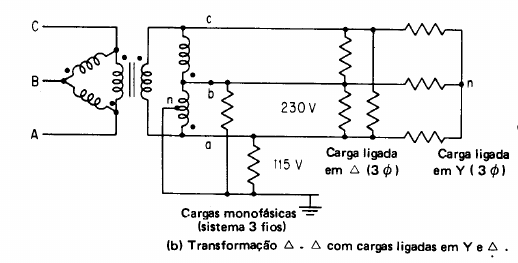
\includegraphics[scale=.8]{TT.png}
    \caption{Ligação Triângulo-Triângulo com cargas diversas}
    \label{fig:figura1}
\end{figure}

Os seguintes valores foram mensurados para a tensões no primário,

\begin{center}
    \begin{tabular}{c||c}
        $V_1$ & 202.4 [V] \\
        $V_2$ & 202.4 [V] \\
        $V_3$ & 202.4 [V] \\
    \end{tabular}
    \captionof{table}{Valores de tensões para o primário}
\end{center}

A correntes no primário são,

\begin{center}
    \begin{tabular}{c||c}
        $I_1$ & 37 [mA] \\
        $I_2$ & 37 [mA] \\
        $I_3$ & 37 [mA] \\
    \end{tabular}
    \captionof{table}{Valores de corrente no primário}
\end{center}

Com isso é possível obter a potências no primário,

\begin{center}
    \begin{tabular}{c||c}
        $W_1$ & 6 [W] \\
        $W_2$ & 6 [W] \\
        $W_3$ & 6 [W] \\
    \end{tabular}
    \captionof{table}{Potências calculadas}
\end{center}

Com isso é possível obter a potências reativas no primário,

\begin{center}
    \begin{tabular}{c||c}
        $W_1$ & 1 [VAr] \\
        $W_2$ & 1 [VAr] \\
        $W_3$ & 1 [VAr] \\
    \end{tabular}
    \captionof{table}{Reativo consumido no primário}
\end{center}

O fator de potência em vazio do transformador fica: 0.9864 (ind)

A tensão no secundário fica,

\begin{center}
    \begin{tabular}{c||c}
        $V_1$ & 225 [V] \\
        $V_2$ & 225 [V] \\
        $V_3$ & 225 [V] \\
    \end{tabular}
\captionof{table}{Tensões no secundário}
\end{center}


\subsection{Ligação Triângulo - Estrela}

Aplica-se uma tensão nos terminais de alta tensão(H1 H2 H3), aumentando gradativamente
a tensão da fonte. Sendo feito a monitoração pelos voltímetros analógicos disponíveis
nos laboratórios.  


Os seguintes valores foram mensurados para a tensões no primário,

\begin{center}
    \begin{tabular}{c||c}
        $V_1$ & 213 [V] \\
        $V_2$ & 213 [V] \\
        $V_3$ & 213 [V] \\
    \end{tabular}
    \captionof{table}{Valores de tensões para o primário}
\end{center}

A correntes no primário são,

\begin{center}
    \begin{tabular}{c||c}
        $I_1$ & 35 [mA] \\
        $I_2$ & 35 [mA] \\
        $I_3$ & 35 [mA] \\
    \end{tabular}
    \captionof{table}{Valores de corrente no primário}
\end{center}

Com isso é possível obter a potências no primário,

\begin{center}
    \begin{tabular}{c||c}
        $W_1$ & 5 [W] \\
        $W_2$ & 5 [W] \\
        $W_3$ & 5 [W] \\
    \end{tabular}
    \captionof{table}{Potências calculadas}
\end{center}

Com isso é possível obter a potências reativas no primário,

\begin{center}
    \begin{tabular}{c||c}
        $W_1$ & 1 [VAr] \\
        $W_2$ & 1 [VAr] \\
        $W_3$ & 1 [VAr] \\
    \end{tabular}
    \captionof{table}{Reativo consumido no primário}
\end{center}

O fator de potência em vazio do transformador fica: 0.9806 (ind)

A tensão no secundário fica,

\begin{center}
    \begin{tabular}{c||c}
        $V_1$ & 122 [V] \\
        $V_2$ & 122 [V] \\
        $V_3$ & 122 [V] \\
    \end{tabular}
\captionof{table}{Tensões no secundário}
\end{center}

\end{document}

